\documentclass[runningheads]{llncs}

\usepackage[T1]{fontenc}
\usepackage{graphicx}
\usepackage{amsmath,amssymb}
\usepackage{algorithm}
\usepackage{algorithmic}
\usepackage{url}
\usepackage{xcolor}
\usepackage[version=4]{mhchem}
\usepackage{siunitx}
\usepackage{cite}
\usepackage{microtype}

\begin{document}

\title{A hybrid ANN-HHO approach for ICE Emission Data Modelling}
\titlerunning{Hybrid ANN-HHO for ICE Emission Data Modelling}

\author{Gabriel Choong Ge Liang\orcidID{0009-0000-8258-2996} \and
Hakim Abdulrab\orcidID{0000-0001-7180-7942}}

\authorrunning{G. Choong and H. Abdulrab}

\institute{School of Artificial Intelligence and Robotics, Xiamen University Malaysia,\\
Sepang, Selangor, Malaysia}

\maketitle

\begin{abstract}
	Road transportation remains a primary contributor to global greenhouse gas emissions, where
	accurate Internal Combustion Engine (ICE) emission modeling is critical for powertrain
	calibration. However, the multi-target prediction of Nitrogen Oxides ($\ce{NO_x}$) and Carbon
	Dioxide ($\ce{CO2}$) involves severe physical trade-offs: $\ce{NO_x}$ kinetics follow exponential
	Arrhenius sensitivity to peak temperature, producing heavy-tailed distribution bursts, whereas
	$\ce{CO2}$ maps quadratically to vehicle specific power. Conventional manual calibration of Feedforward
	Neural Networks fails under these opposing dynamics; human-tuned learning rate schedulers
	(e.g., StepLR) overfit the smoother $\ce{CO2}$ trajectory while collapsing $\ce{NO_x}$ fidelity
	to severe overfitting. In this study, we propose a hybrid Artificial Neural Network and Harris
	Hawks Optimization (ANN-HHO) framework for multi-target vehicle emission modeling, predicting
	$\ce{NO_x}$ and $\ce{CO2}$ simultaneously from OBD-II telemetry driving data. Our framework
	employs a compute-restricted proxy objective ($E_{\text{proxy}} \le 20$ epochs) to prevent
	premature weight memorization while discovering global optimal topologies and flat optimizers. The
	unrestricted model (HHO-UR) achieves superior predictive fidelity with an $R^2$ of $0.9823$ for
	$\ce{NO_x}$ and $0.9950$ for $\ce{CO2}$, decisively resolving the generalization failure observed
	in the manual baseline model ($R^2 = 0.5714 \pm 0.2240$). Furthermore, under a restricted
	budget ($\le 20$ epochs), restricted HHO (HHO-R) attains an $88.7\%$ reduction in training epochs
	(17 vs. 150) with an $R^2$ of $0.9327$, cutting search wall-clock duration from 9.1 hours to 76
	minutes. Comparative evaluation against alternative metaheuristics (PSO, ACOR, and SCA) confirms
	that the HHO framework consistently discovers compact, generalizable two-layer topologies,
	demonstrating a scalable and computationally efficient methodology for intelligent automotive engine management.

	\keywords{Internal combustion engines \and Vehicle emission modeling \and Multi-target prediction
	\and Artificial neural networks \and Harris Hawks optimization \and OBD-II telemetry.}
\end{abstract}

\section{Introduction}
The Internal Combustion Engine is the backbone of modern society. Rapid adoption of passenger vehicles throughout the
20\textsuperscript{th} and 21\textsuperscript{st} century uncovered the fundamental downside of the combustion process.
The chemical reaction of igniting fossil fuels in the presence of air under high temperature and high pressure releases
significant quantities of greenhouse gases responsible for global warming such as nitrogen oxides ($\ce{NO_x}$), carbon
dioxide ($\ce{CO2}$), carbon monoxide ($\ce{CO}$) and sulphur dioxide ($\ce{SO2}$).

The effectiveness of manual calibration of ICE systems is inherently limited by the thermodynamics of the combustion
process. In passenger vehicles, the Engine Control Unit (ECU) manages fuel delivery, ignition timing, and air intake to
balance three competing operational objectives: maximizing fuel economy, extracting peak power, and minimizing exhaust
emissions. Due to the high degrees of non-linearity in in-cylinder chemical kinetics, dynamic engine operating
conditions lead to transient emission spikes that fixed empirical lookup tables cannot dynamically mitigate.

Recent advancements in computing power and algorithmic design enabled the integration of Artificial Intelligence (AI)
technologies into automotive powertrains. Data-driven models, such as Artificial Neural Networks (ANNs), have shown
exceptional capability in learning complex, non-linear relationships across high-dimensional input spaces without
requiring closed-form physical calibrations. In particular, ANNs have been increasingly adopted to model physical engine
characteristics, replacing computationally expensive Fluid Dynamics (CFD) simulations and costly physical dynamometer
testing. Neural network architectures have demonstrated high fidelity in approximating emissions, with applications
ranging from predictive emissions monitoring systems (PEMS) to real-time engine control
\cite{weteringArtificialNeuralNetworkBased2023, nitrogenDioxideThermalDecomposition,
modelingNonlinearRelationships}.

Despite these promising applications, training ANNs for multi-target vehicle emission modeling introduces significant
mathematical hurdles. The emission of $\ce{NO_x}$ and $\ce{CO2}$ operate on radically different physical mechanisms:
while $\ce{CO2}$ is primarily a function of fuel consumption and vehicle specific power, $\ce{NO_x}$ formation is
exponentially sensitive to peak combustion temperatures and local oxygen concentrations via the thermal Zeldovich
mechanism. When optimizing a shared neural network representation, standard backpropagation struggles to escape local
extrema, often sacrificing the prediction fidelity of one pollutant to minimize the loss of another. Furthermore,
manual hyperparameter tuning of these networks is prone to human bias, frequently yielding oversized architectures that
suffer from severe overfitting or excessive computational latency incompatible with embedded ECU deployment.

To address these challenges, this study proposes a hybrid Artificial Neural Network and Harris Hawks Optimization
(ANN-HHO) framework for multi-target vehicle emission modeling. By integrating nature-inspired metaheuristic search into
the architectural design and hyperparameter selection process, the proposed framework automates the discovery of
optimal network topologies, learning dynamics, and regularization schemes. The primary contributions of this work are
threefold:
\begin{enumerate}
	\item We develop a unified multi-target prediction pipeline that models $\ce{NO_x}$ and $\ce{CO2}$ emissions
		simultaneously using vehicle on-board diagnostics (OBD-II) telemetry, demonstrating that nature-inspired heuristics
		effectively resolve the multi-objective optimization tension between chemically divergent pollutants.
	\item We introduce an epoch-constrained proxy evaluation strategy within the metaheuristic search loop, enabling the
		rapid exploration of the hyperparameter space while preventing the optimization algorithm from converging toward
		over-parameterized models that exhibit memorization.
	\item We benchmark the proposed HHO-optimized framework against both a manually tuned baseline and multiple
		state-of-the-art metaheuristic algorithms (Particle Swarm Optimization, Ant Colony Optimization for Continuous
		Domains, and the Sine Cosine Algorithm), providing a rigorous empirical evaluation of predictive accuracy, model
		compactness, and search convergence efficiency.
\end{enumerate}

\section{Related Works}

The integration of artificial intelligence and machine learning into internal combustion engine modeling has seen
rapid expansion over the past decade. Traditional phenomenological and zero-dimensional thermodynamic models, while
computationally lightweight, often lack the precision required for transient emission estimation. Conversely,
three-dimensional computational fluid dynamics (CFD) simulations offer high physical fidelity but are prohibitively
expensive for real-time engine calibration or iterative design space exploration. Data-driven surrogate models have
emerged as a viable middle ground, offering near-instantaneous inference with minimal accuracy loss.

Artificial Neural Networks (ANNs) have been widely deployed to predict critical engine performance metrics, including
thermal efficiency, brake torque, and specific fuel consumption, alongside exhaust emissions across varying fuel
blends and engine load cycles \cite{bhattApplicationArtificialNeural2022, tuanhoangReviewApplicationArtificial2021}.
Recent efforts in ICE optimization for lowering emissions leveraging ANNs have proven to reduce developmental time and
flexibility of these neural networks \cite{karunamurthyPredictionICEngine2023,
inezahavugimanaReviewArtificialIntelligent2023}. Several studies confirmed the reliability of pairing an ANN with
optimization algorithms to design a mathematically optimal network architecture
\cite{sharmaApplicationMachineLearning2023, usluOptimizationDieselEngine2020, singhSampleddataModelValidation2020}. The
application of optimization algorithms on ANNs demonstrated a better performance overall for training a model on IC
Engine telemetry \cite{gunawanApplicationArtificialNeural2024} when compared to manual-tuned ANNs.

Nature-inspired swarm heuristics reliably navigate non-convex engineering landscapes.
Specifically, Harris Hawks Optimization (HHO)~\cite{heidariHarrisHawksOptimization2019} alternates
between exploratory perching and Levy-flight-driven dives to satisfy sensor coverage and sink-node
routing constraints in industrial networks~\cite{abdulrab2022optimal, abdulrab2022hho}.
At the powertrain layer, reinforcement learning policies have proven effective for non-linear Engine
Control Unit (ECU) calibration~\cite{omranDeepReinforcementLearning2024}.
Applying similar population-based exploration enables neural surrogate models to approximate
rugged internal combustion engine emission data without trapped trajectories in poor local minima.

\section{Proposed Methodology}

\subsection{Nitrogen Oxides $\ce{NO_x}$ Approximation}\label{sec:nox-modelling}

Nitrogen Oxides ($\ce{NO_x}$) are notorious for being difficult to predict in a combustion process using pure
mathematical models. The common way of predicting $\ce{NO_x}$ is to use a supervised-learning algorithm to achieve
relatively high accuracy. Nitrogen Oxide ($\ce{NO}$) has a formation rate \cite{THOMPSON1973787} of

\begin{equation}
	\frac{d[NO]}{dt} = 1.503 \times 10 \cdot T^{-0.5} \cdot [O_2]^{0.5}
	\cdot [N_2] \cdot \frac{[O]}{[O]\textsubscript{eq}} \cdot e^{\frac{-134.7}{RT}}
	\label{eqn:no-rate}
\end{equation}
where $T$ is temperature [K], $[O]\textsubscript{eq}$ equilibrium atomic oxygen concentration, and
$R$ is the ideal gas constant [J/mol$ \cdot $K].
From \eqref{eqn:no-rate},
\begin{equation}
	\ce{NO_x} = \int_{0}^{t} f(T, [\ce{O_2}], [\ce{N_2}], [O], [O]\textsubscript{eq}) \quad dt
	\label{eqn:nox-integral}
\end{equation}
The combustion process of the IC Engine that releases $\ce{NO_x}$ consists of Nitrogen Dioxide ($\ce{NO2}$) and
Nitrogen Monoxide ($\ce{NO}$). $\ce{NO2}$ can be assumed to decay into $\ce{NO}$ via thermal decomposition:
\begin{equation}
	2\ce{NO2} \rightarrow 2\ce{NO} + \ce{O2}
	\label{eq:no2tono}
\end{equation}
The generation of $\ce{NO_x}$ emission from an IC engine can then be estimated by:
\begin{equation}
	\ce{NO_x} \approx a \cdot \text{RPM} + b \cdot \text{LOAD} + c \cdot \text{COOLANT\_TEMP} + d \cdot \text{IAT}
	\label{eqn:nox-estimate}
\end{equation}

\subsection{Carbon Dioxide $\ce{CO2}$ Approximation}\label{sec:co(-_2-)-modelling}

Vehicle Specific Power (VSP) represents the instantaneous power demand of the engine per unit of vehicle mass.
VSP is calculated as:
\begin{equation}
	\text{VSP} = v \cdot (1.1 \cdot a + 9.81 \cdot \text{grade} + 0.132) + 0.000302 \cdot v^3
	\label{eq:vsp}
\end{equation}
where $v$ is vehicle speed (m/s), $a$ is vehicle acceleration ($\text{m/s}^2$), and $\text{grade}$ is the road gradient
in percentage. Since driving on flat roads is assumed, $\text{grade} = 0$.

$\ce{CO2}$ emission is closely related to fuel consumption and engine load. An empirical model correlates VSP with
$\ce{CO2}$ emission rate \cite{CHEN2024133892}:
\begin{equation}
	\ce{CO2} = 0.00995 \cdot \text{VSP}^2 + 0.2573 \cdot \text{VSP} + 1.443
	\label{eqn:co2_and_vsp}
\end{equation}

\begin{algorithm}[t]
	\caption{Proposed Metaheuristic Neural Architecture and Hyperparameter Optimization}
	\label{alg:metaheuristic_optimization}
	\begin{algorithmic}[1]
		\REQUIRE Training set $\mathcal{D}_{\text{train}}$, validation set $\mathcal{D}_{\text{val}}$,
		population size $N_p = 15$, search iterations $T_{\max} = 5$, metaheuristic operator $\mathcal{M}
		\in \{\text{ACOR}, \text{PSO}, \text{HHO}, \text{SCA}\}$, parameter bounds $\mathbf{\Omega}$.
		\ENSURE Optimal configuration $\mathbf{x}^*$, evaluated surrogate model $\mathcal{F}_{\mathbf{x}^*}$.

		\STATE \textbf{Initialize:} Population $\mathbf{P}^{(0)} = \{\mathbf{x}_1, \dots,
		\mathbf{x}_{N_p}\} \sim \mathcal{U}(\mathbf{\Omega})$, global minimum fitness $f^* \leftarrow \infty$.

		\FOR{iteration $t = 1$ \TO $T_{\max}$}
		\FOR{each candidate solution $\mathbf{x}_i \in \mathbf{P}^{(t-1)}$}
		\STATE Decode $\mathbf{x}_i \to \{L, [u_1, \dots, u_L], \sigma, \mathcal{O}, E_{\text{proxy}}, B\}$.
		\STATE Instantiate FNN $\mathcal{F}_{\mathbf{x}_i}$ with $L$ layers, hidden units $u_l$, and activation $\sigma$.
		\STATE Configure optimizer $\mathcal{O}$ with learning rate $\eta = 0.001$.
		\STATE Partition $\mathcal{D}_{\text{train}}$ into mini-batches of size $B$.

		\FOR{epoch $e = 1$ \TO $E_{\text{proxy}}$}
		\FOR{each mini-batch $(\mathbf{X}_b, \mathbf{y}_b) \in \mathcal{D}_{\text{train}}$}
		\STATE $\hat{\mathbf{y}}_b \leftarrow \mathcal{F}_{\mathbf{x}_i}(\mathbf{X}_b)$
		\STATE $\mathcal{L} \leftarrow \frac{1}{|\mathbf{X}_b|} \|\hat{\mathbf{y}}_b - \mathbf{y}_b\|_2^2$ \COMMENT{MSE Loss}
		\STATE $\mathbf{W} \leftarrow \mathbf{W} - \eta \nabla_{\mathbf{W}} \mathcal{L}$
		\ENDFOR
		\ENDFOR

		\STATE Forward validation pass: $\hat{\mathbf{Y}}_{\text{val}} \leftarrow
		\mathcal{F}_{\mathbf{x}_i}(\mathbf{X}_{\text{val}})$.
		\STATE Compute coefficient of determination: \\
		\quad $R^2 \leftarrow 1 - \frac{\sum_{j} (\mathbf{y}_{\text{val}, j} -
		\hat{\mathbf{y}}_{\text{val}, j})^2}{\sum_{j} (\mathbf{y}_{\text{val}, j} - \bar{\mathbf{y}}_{\text{val}})^2}$.
		\STATE Assign fitness: $f(\mathbf{x}_i) \leftarrow 1 - R^2$.

		\IF{$f(\mathbf{x}_i) < f^*$}
		\STATE $f^* \leftarrow f(\mathbf{x}_i)$, \quad $\mathbf{x}^* \leftarrow \mathbf{x}_i$.
		\ENDIF
		\ENDFOR
		\STATE Update population positions: $\mathbf{P}^{(t)} \leftarrow \mathcal{M}(\mathbf{P}^{(t-1)}, \mathbf{x}^*)$.
		\ENDFOR

		\STATE \textbf{Stage-2 Evaluation:} Evaluate $\mathcal{F}_{\mathbf{x}^*}$ on held-out test
		telemetry $\mathcal{D}_{\text{test}}$ to record generalization metrics.
		\RETURN $\mathbf{x}^*, \mathcal{F}_{\mathbf{x}^*}$.
	\end{algorithmic}
\end{algorithm}

\subsection{Two-Stage Metaheuristic Neural Architecture Search}

The proposed optimization framework operates on a Two-Stage Neural Architecture Search (NAS)
paradigm, formalized in Algorithm~\ref{alg:metaheuristic_optimization}. Rather than evaluating
arbitrarily deep network topologies over exhaustive training cycles, the continuous search vector
$\mathbf{x} \in \mathbf{\Omega}$ dynamically parameterizes both network capacity (number of layers
	$L \in [1, 5]$, unit width per layer $u_l \in [2, 256]$, and activation $\sigma \in \{\text{ReLU},
\text{Sigmoid}\}$) and the gradient descent dynamics (optimizer $\mathcal{O}$, batch size $B \in
[16, 64]$, and proxy epoch budget $E_{\text{proxy}} \le 20$).

During Stage-1 search, candidate architectures train under a restricted proxy budget using standard
Mean Squared Error (MSE) loss, mapping validation performance to the minimization objective
$f(\mathbf{x}) = 1 - R^2$. Population vectors update iteratively via operator $\mathcal{M}$ across
ACOR, AIW-PSO, standard HHO, or Dev-SCA. We include Dev-SCA alongside HHO because coupled
trigonometric and arithmetic operators~\cite{abdulrab2023hybrid, devan2023novel, abdulrab2024energy}
maintain step-size diversity and escape saddle points across non-convex parameter landscapes.
All algorithmic routines and parameter bounds run within the MEALPY
library~\cite{van2023mealpy,van2023groundwater,ahmed2021comprehensive}. Once the population
converges, Stage-2 isolates the global optimum $\mathbf{x}^*$, benchmarking its out-of-sample
test generalization directly against the manual baseline model.

\section{Results}

\subsection{Metaheuristic Optimization Benchmark}

The predictive performance and computational efficiency of the neural architectures discovered
across all four metaheuristic algorithms, namely Ant Colony Optimization for Continuous Domains (ACOR),
Adaptive Inertia Weight Particle Swarm Optimization (AIW-PSO), Harris Hawks Optimization (HHO), and
the Sine Cosine Algorithm (SCA), were comprehensively evaluated against the manual baseline model.
Table~\ref{tab:master_benchmark} reports the test metrics, discovered topologies, and search
overhead across all evaluated models.

\begin{table}[t]
	\centering
	\caption{Comprehensive Performance and Computational Comparison: Manual Baseline vs. Metaheuristic-Optimised Models}
	\label{tab:master_benchmark}
	\setlength{\tabcolsep}{3.5pt}
	\resizebox{\textwidth}{!}{%
		\begin{tabular}{lccccccc}
			\hline
			\textbf{Model / Heuristic} & \textbf{Network Topology} & \textbf{Epochs} & \textbf{Optimizer} &
			\textbf{Test Loss} & \textbf{$R^2$ (NO\textsubscript{x})} & \textbf{$R^2$ (CO\textsubscript{2})}
			& \textbf{Search Time} \\
			\hline
			\textbf{Manual Baseline} & $[32, 32, 16]$ (3 layers) & 150 & Adam + StepLR & $97.12 \pm 25.01$ &
			$0.5714 \pm 0.224$ & \textbf{0.9992} $\pm$ 0.0002 & N/A \\
			\textbf{SCA} & $[94, 202]$ (2 layers) & \textbf{15} & RMSprop & 1188.31 & 0.8988 & 0.9884 & \textbf{48.5 min} \\
			\textbf{HHO-R (Restricted)} & $[138, 256]$ (2 layers) & \textbf{17} & Nadam & 678.81 & 0.9327 & 0.9934 & 76.1 min \\
			\textbf{PSO} & $[242, 125]$ (2 layers) & \textbf{20} & Nadam & 1214.30 & 0.9817 & 0.9882 & \textbf{57.0 min} \\
			\textbf{ACOR (Lowest Loss)} & $[205, 256]$ (2 layers) & \textbf{20} & Adam & \textbf{590.71} &
			0.9793 & 0.9942 & 101.7 min \\
			\textbf{HHO-UR (Unrestricted)} & $[175, 211, 220, 242, 21]$ (5 layers) & 150 & RMSprop & 514.35 &
			\textbf{0.9823} & 0.9950 & 543.8 min (9.1h) \\
			\hline
		\end{tabular}%
	}
\end{table}

For $E_{\text{proxy}} \le 20$ epochs, metaheuristic optimisation yielded consistent improvements in $R^2$ over the
manual baseline model, which struggled over the non-linear $\ce{NO_x}$ computed emission data. As shown in
Table~\ref{tab:master_benchmark},
ACOR achieved the lowest test MSE loss of $590.71$ alongside an $R^2$ score of $0.9793$ for
$\ce{NO_x}$ and $0.9942$ for $\ce{CO2}$
in only 20 epochs. AIW-PSO demonstrated strong predictive fidelity, yielding an
$R^2$ of $0.9817$ for $\ce{NO_x}$ and $0.9882$ for $\ce{CO2}$ with a test loss of $1214.30$, while
completing its Stage-1 search in the shortest duration among high-performing variants ($57.0$
minutes). Restricted HHO (HHO-R) converged at 17 epochs with an $R^2$ of $0.9327$ for $\ce{NO_x}$
and $0.9934$ for $\ce{CO2}$ with a test loss of $678.81$ in $76.1$ minutes. Even SCA, the most
computationally lightweight
optimiser ($48.5$ minutes search), achieved an $R^2$ of $0.8988$ for $\ce{NO_x}$ and $0.9884$ for
$\ce{CO2}$ in only 15 epochs.

\begin{table}[htbp]
	\centering
	\caption{Metaheuristic Optimization Benchmark under Restricted Training Regime ($\le 20$ Epochs)}
	\label{tab:metaheuristic_benchmark}
	\setlength{\tabcolsep}{5pt}
	\resizebox{0.95\textwidth}{!}{%
		\begin{tabular}{lcccc}
			\hline
			\textbf{Algorithm} & \textbf{Best Topology} & \textbf{Epochs} & \textbf{Search $R^2$ (\%)} &
			\textbf{Search Time} \\
			\hline
			ACOR & $[205, 256]$ (2 layers) & 20 & \textbf{89.21\%} & 101.7 min \\
			PSO & $[242, 125]$ (2 layers) & 20 & 88.95\% & \textbf{57.0 min} \\
			HHO & $[138, 256]$ (2 layers) & 17 & 88.91\% & 76.1 min \\
			SCA & $[94, 202]$ (2 layers) & 15 & 82.28\% & \textbf{48.5 min} \\
			\hline
		\end{tabular}%
	}
\end{table}

By contrast, the manual baseline model ($[32, 32, 16]$ with Adam and StepLR) achieved a
respectable $R^2$ of $0.9992 \pm 0.0002$ for $\ce{CO2}$, but exhibited severe instability on
$\ce{NO_x}$, collapsing to an average $R^2$ of $0.5714 \pm 0.2240$ (with individual experimental
runs dropping as low as $0.3117$). Furthermore, unconstrained HHO (HHO-UR), which allowed 150
training epochs and up to 5 hidden layers, attained an $R^2$ of $0.9823$ for $\ce{NO_x}$ and
$0.9950$ for $\ce{CO2}$ at a test loss of $514.35$. However, this marginal gain over restricted
ACOR required $543.8$ minutes ($9.1$ hours) of search wall-clock time, representing a more than five-fold
increase in compute overhead. Figure~\ref{fig:comparative_performance} provides a visual synthesis
of these accuracy gains and computational trade-offs.

\begin{figure}[htbp]
	\centering
	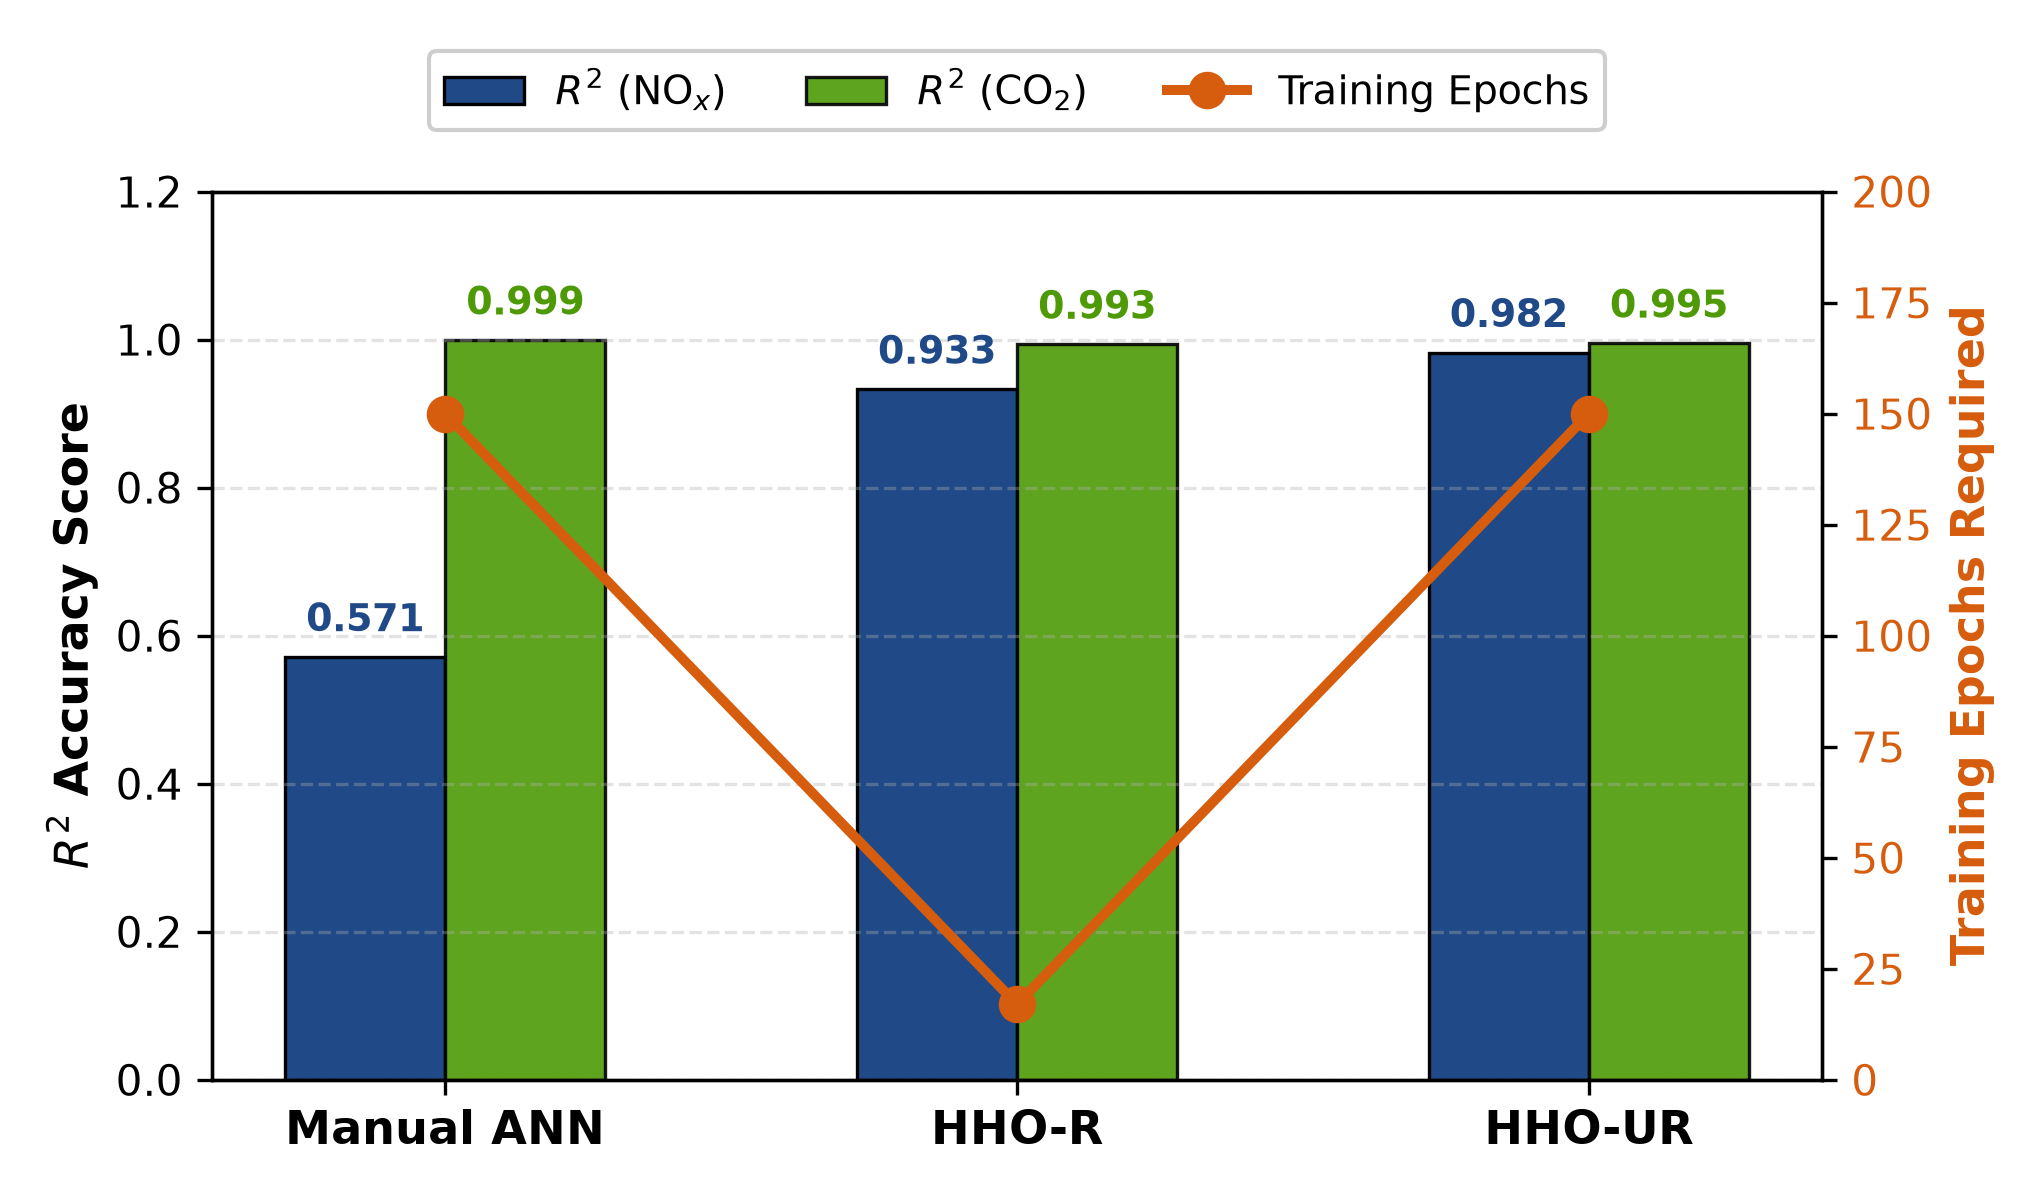
\includegraphics[width=0.75\textwidth]{images/comparative_performance_chart.png}
	\caption{Performance and epoch requirements for the baseline vs. metaheuristic models on $\ce{NO_x}$ and
	$\ce{CO2}$.}
	\label{fig:comparative_performance}
\end{figure}

Table~\ref{tab:metaheuristic_benchmark} shows that the ranking of the algorithms remain identical between the Stage-1
proxy search ($1 - R^2$) and the Stage-2 evaluation:
\begin{equation}
	\text{ACOR} \succ \text{PSO} \succ \text{HHO-R} \succ \text{SCA} \gg \text{Manual Baseline}.
\end{equation}
This confirms that a short $\le 20$ epoch training constraint reliably identifies the best architectures without wasting
compute on 150 epochs during search.

\subsection{Convergence Dynamics and Compute Budget Savings}

Figure~\ref{fig:loss_convergence_comparison} shows the training loss convergence trend for the
optimization algorithms. In Figure~\ref{fig:loss_convergence_comparison}(a), rapid error reduction
is observed for all metaheuristic algorithms within the 20 epoch limit. The final losses settled
just below the $1000$ mark around the 15\textsuperscript{th} epoch. ACOR showed the steepest initial
descent to under $2000$ by the 6\textsuperscript{th} epoch due to its smaller mini-batch size ($B =
16$) and frequent stochastic weight updates. PSO achieved the lowest training loss among epoch
limited training at $568$ by epoch 20.

\begin{figure}[t]
	\centering
	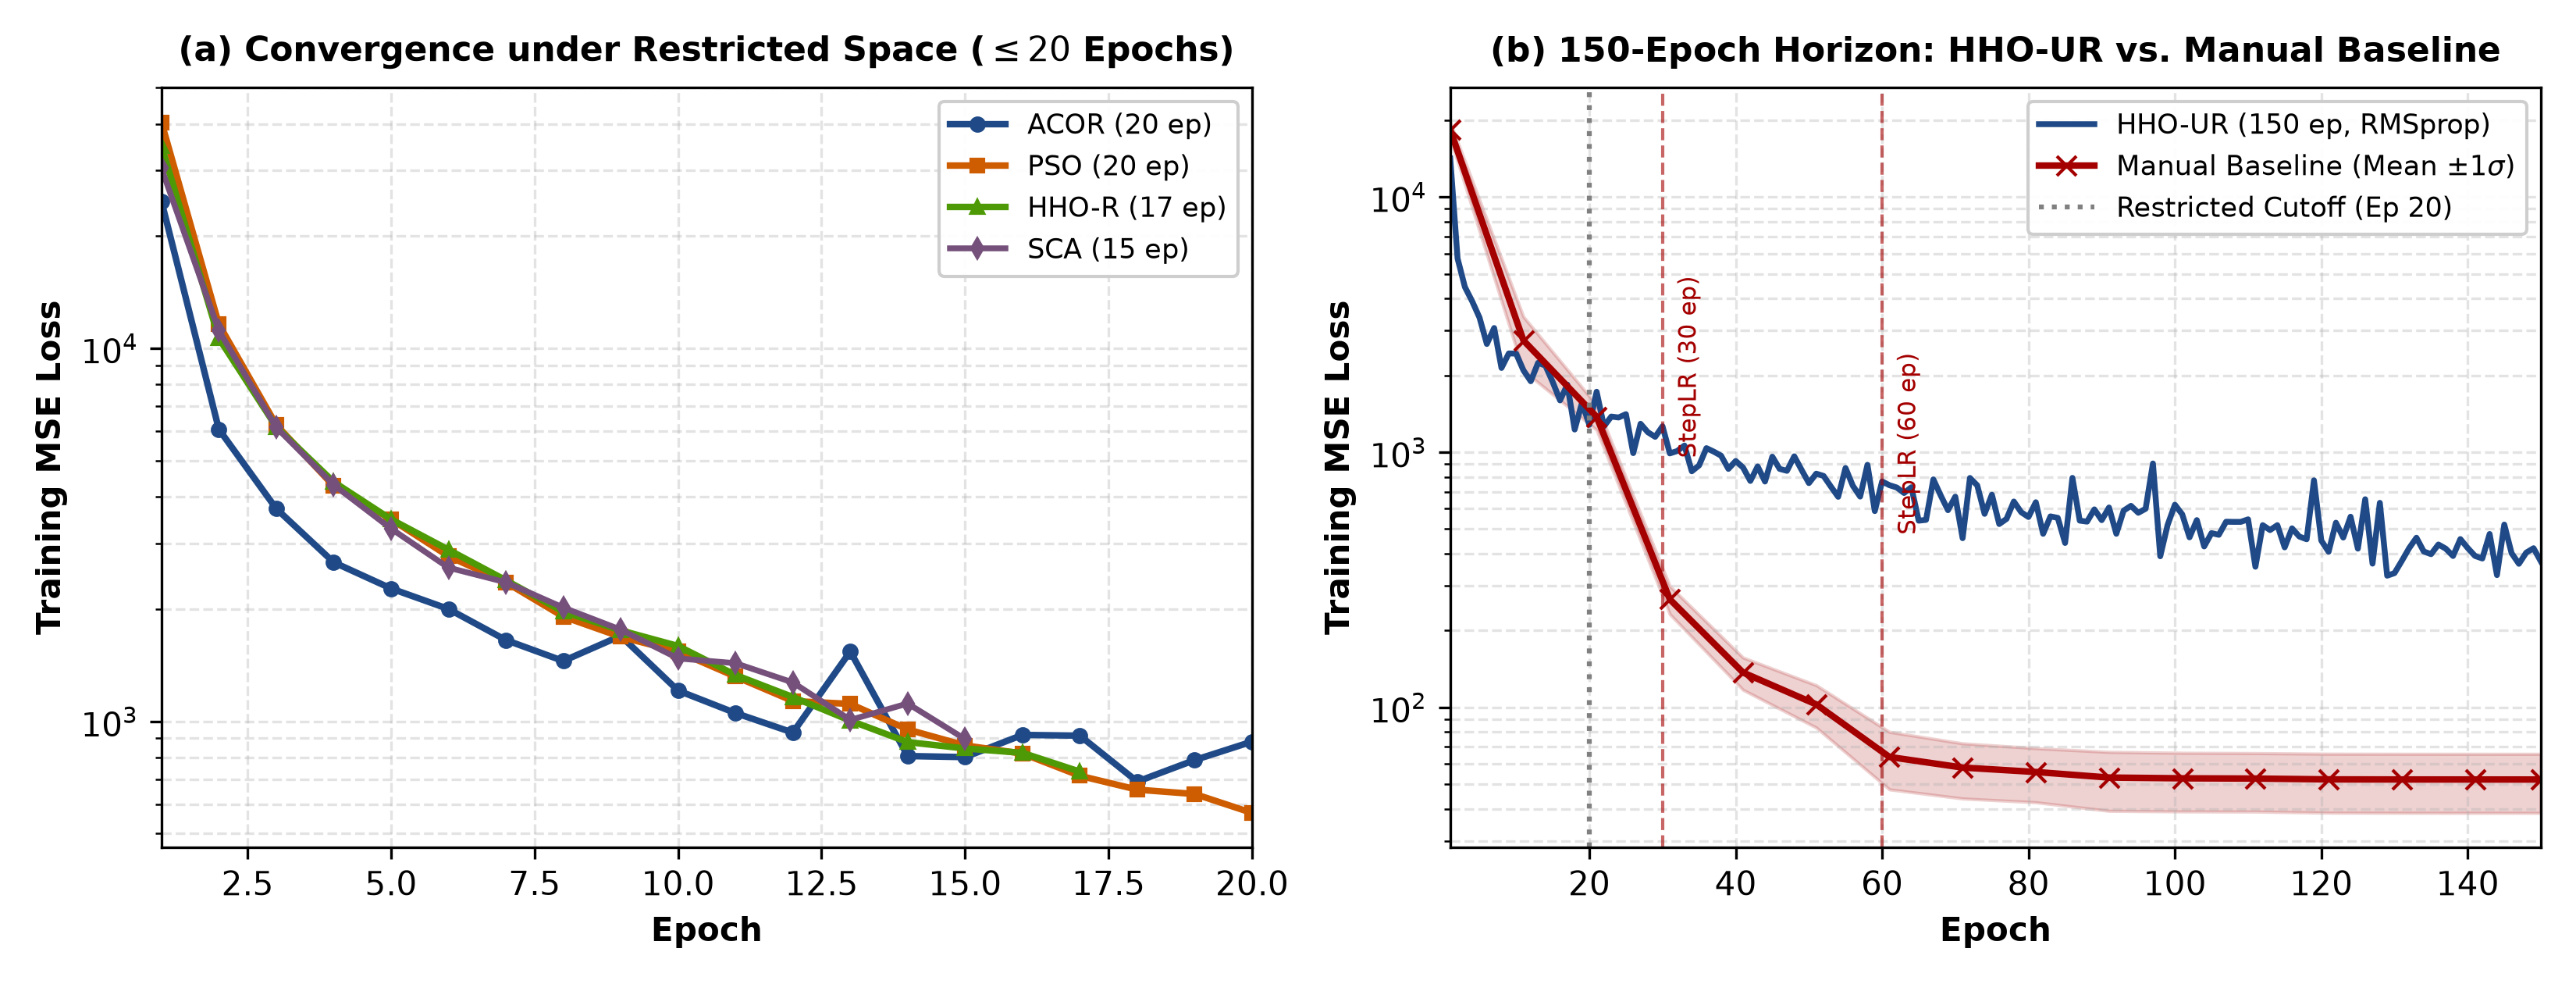
\includegraphics[width=\textwidth]{images/loss_convergence_comparison.png}
	\caption{Training loss convergence dynamics: (a) Rapid log-linear error reduction of
		metaheuristic-optimised architectures within the restricted budget ($\le 20$ epochs); (b)
		150-epoch extended training horizon comparing HHO-UR against the manually tuned baseline,
	highlighting the artificial loss suppression from StepLR decay at epochs 30 and 60.}
	\label{fig:loss_convergence_comparison}
\end{figure}

\begin{table}[htbp]
	\centering
	\caption{Performance and Computational Comparison: Baseline vs. Restricted and Unrestricted HHO}
	\label{tab:hho_comparison}
	\setlength{\tabcolsep}{4pt}
	\resizebox{0.95\textwidth}{!}{%
		\begin{tabular}{lccc}
			\hline
			\textbf{Metric / Hyperparameter} & \textbf{Manual Baseline} & \textbf{HHO-R (Restricted)} &
			\textbf{HHO-UR (Unrestricted)} \\
			\hline
			Topology & $[32, 32, 16]$ (3L) & $[138, 256]$ (2L) & $[175, 211, 220, 242, 21]$ (5L) \\
			Total Hidden Neurons & 80 & 394 & 869 \\
			Epochs & 150 & \textbf{17} & 150 \\
			Compute Budget (\% Epochs) & 100\% & \textbf{11.3\%} & 100\% \\
			Batch Size & 32 & 40 & 64 \\
			Optimizer & Adam + StepLR & Nadam (Flat) & RMSprop (Flat) \\
			$R^2$ (CO\textsubscript{2}) & \textbf{0.9992} $\pm$ 0.0002 & 0.9934 & 0.9950 \\
			$R^2$ (NO\textsubscript{x}) & 0.5714 $\pm$ 0.2240 & \textbf{0.9327} & \textbf{0.9823} \\
			Evaluation Loss & $97.12 \pm 25.01$ & 678.81 & 514.35 \\
			Search Wall-Clock Time & N/A & \textbf{1h 16m} & 9h 04m \\
			\hline
		\end{tabular}%
	}
\end{table}

Figure~\ref{fig:loss_convergence_comparison}(b) highlights the fundamental behavioral divide across the extended
150-epoch horizon, comparing HHO-UR against the manual baseline model across five independent trials. The manual
baseline displays distinct loss drop-offs at epoch 30 and epoch 60, corresponding exactly to scheduled StepLR
learning-rate decays ($\gamma = 0.1$). Although these step decays drive the final training MSE down
to $97.12 \pm 25.01$,
they force the optimizer into narrow, non-generalizable minima. Consequently, test-set evaluation reveals severe
overfitting on the non-linear $\ce{NO_x}$ target ($R^2 = 0.5714 \pm 0.2240$, with individual runs dropping as low as
$0.3117$).

In contrast, HHO-UR maintained smooth, continuous loss progression without artificial learning-rate shocks. While its
final MSE appears higher on training curves ($514.35$), it achieved superior out-of-sample generalization across both
targets ($R^2 = 0.9823$ for $\ce{NO_x}$ and $0.9950$ for $\ce{CO2}$). Furthermore, as detailed in
Table~\ref{tab:hho_comparison}, the compute-constrained HHO-R variant discovered a lean two-layer topology ($[138,
256]$) that converged in just 17 epochs (76.1 minutes), capturing $94.9\%$ of HHO-UR's $\ce{NO_x}$ performance while
slashing training epoch overhead by $88.7\%$.

\subsection{Architectural Regularization: Shallow-Wide vs. Deep-Narrow Topologies}

A key qualitative insight from the optimization benchmarks is the structural morphology of the discovered networks.
Across all four metaheuristic algorithms, the search consistently converged on shallow-wide representations (two hidden
layers: $[205, 256]$ for ACOR, $[242, 125]$ for PSO, $[138, 256]$ for HHO, and $[94, 202]$ for SCA). The widened first
hidden layer ($> 94$ units, scaling up to 242 units in PSO) acts as a high-dimensional feature expansion mechanism,
allowing the network to disentangle linear vehicle kinetics ($\ce{CO2}$) from the severe non-linearities of thermal
formation ($\ce{NO_x}$) before projection into the secondary layer.

Conversely, deeper architectures evaluated during unrestricted search (such as HHO-UR's five-layer $[175, 211, 220,
242, 21]$ configuration) yielded only marginal improvements in $R^2$ ($+0.0496$ on $\ce{NO_x}$) at the expense of a
$5.7\times$ increase in parameter volume and an exponential increase in training wall-clock time. This demonstrates that
for tabular OBD-II telemetry streams, over-parameterized deep architectures provide diminishing returns over well-tuned
two-layer wide networks.

\subsection{Hyperparameter Sensitivity: Flat vs. Decaying Learning Rate Schedules}

The experimental findings underscore the critical role of optimization dynamics over raw layer depth. The manual
baseline model utilized a StepLR scheduler that decayed the learning rate from $10^{-2}$ to $10^{-4}$ across 150
epochs. While this produced a deceptive drop in training loss, the rapid decay restricted parameter mobility before the
network could escape local saddles in the $\ce{NO_x}$ error surface, inducing severe generalization collapse (test $R^2$
stalled at $0.5714$).

In contrast, the metaheuristically discovered models employed adaptive, flat optimizers (Adam, Nadam, RMSprop) without
aggressive scheduler decay, coupled with wider hidden layer representations. This allowed the models to escape shallow
local extrema and converge toward flatter, generalizable minima, securing test $R^2$ scores above $0.93$ for $\ce{NO_x}$
and $0.99$ for $\ce{CO2}$ in under 20 epochs.

\subsection{Discussion}

The usage of metaheuristic algorithms highlights the limitations of manual hyperparameter tuning in
a non-linear dataset. Since both target variables were computed according to the equations in
Sections~\ref{sec:co(-_2-)-modelling} and~\ref{sec:nox-modelling}, we could deduce that the model
converged for the mathematical approximations of both target variables. More specifically,
$\ce{NO_x}$ approximations include the Boltzmann factor which makes it harder to generalise in
addition to the $\ce{CO2}$ approximation which is a quadratic computation over $VSP$. This is
reflected clearly in Table~\ref{tab:master_benchmark} where the manual baseline model underfitted
and overfitted simultaneously over the two targets.

In addition, Equation~\ref{eqn:nox-estimate} assumed four tunable coefficients $a,b,c,d$. However, it
was assumed as $a=b=c=d=1$ in the experiments as a basis for the model since this paper aim to
highlight the effectiveness of a hybrid ANN-Heuristic model, in which it can be assumed as a
constant.

The proposed methodology could be applied to a wide range of engineering problems, primarily IC
engine design as the main focus of this paper. The next generation of automotive vehicles have
increasingly stringent emission rules to comply with. Aiding with the design process, critical
emission targets could be mapped using approximation formulae and guardrail the design process
before testing the physical prototype.

\section{Conclusion and Future Works}

This study demonstrated that pairing artificial neural networks with metaheuristic optimization
(ANN-HHO) delivers high-fidelity surrogate modeling for internal combustion engine emissions while
eliminating manual trial-and-error bottlenecks. Under compute-restricted proxy evaluations ($\le 20$
epochs), metaheuristically discovered architectures converged on robust, shallow-wide topologies (two
layers, $\ge 138$ units), decisively preventing the scheduler-induced overfitting that degraded the
manual baseline ($R^2 = 0.5714 \pm 0.2240$). Specifically, HHO-UR attained top $\ce{NO_x}$ fidelity
($R^2 = 0.9823$), while HHO-R achieved an $88.7\%$ reduction in training epochs (17 versus 150) and
reduced search runtime down to 76 minutes.

Further research can experiment on adapting the ANN-HHO model in the Engine Control Unit (ECU)
hardware algorithm design. Applications of the proposed methodology shall not only be limited to
emission reduction, but also the inclusion of other design goals such as closing the gap between the
theoretical and actual maximum power extraction, or engineering challenges of the current ICE
landscape.

\subsubsection*{Data and Code Availability}
The OBD-II telemetry driving logs analyzed in this study are openly accessible via~\cite{cephasax_obdii_ds3}.
To facilitate reproducibility, the complete neural architecture search pipeline, baseline calibration
routines, and trained surrogate models will be made publicly available upon conference publication.

\bibliographystyle{splncs04}
\bibliography{ref/references,ref/nox,ref/co2}

\end{document}
